\documentclass[../tesi.tex]{subfiles}
\begin{document}

\chapter{Analisi dei Casi di Studio}
\section{Introduzione}
L’obiettivo di questo capitolo è provare a trovare un invariante generica tra i diversi workflow riguardanti i case study trovati, e la difficoltà del lavoro sta proprio nel cercare di mettere insieme le varie ricerche nonostante siano molto diverse tra loro.\\
I case study trovati, insieme ai compagni di corso Luca Genova e Marco Benito Tomasone sono:
\begin{itemize}
  \item IA nel campo della radiologia
  \item	Previsione della domanda[Forecasting]
  \item ML nelle reti [Networking]
  \item	IA nel campo della Cybersecurity
  \item Face2Face Traslation
  \item	Recommender System 
\end{itemize}
L’obiettivo è confrontare le tecniche usate in tutti i precedenti case study, cercando di trovare dei punti in comune con la possibilità di evidenziare un workflow il più possibile generico, al fine di adattare e gestire una pipeline di lavoro e individuare in maniera ottimale e automatica il risultato che si va cercando.

\section{Analisi}
In tutti i casi di studio analizzati, anche se molto diversi tra loro abbiamo trovati dei passaggi in comune che andremo ad analizzare singolarmente, rilevando caso per caso le particolarità.
\subsection{Raccolta Dati}
La raccolta dati è fondamentale in ogni processo di apprendimento automatico; spesso si diversifica quando viene effettuata la prima elaborazione.\\
Nonostante i dati risultino in essere molto diversi tra loro, la loro raccolta può trovare dei punti d’accordo.\\
Spesso questi dati vengono suddivisi a seconda della metodologia di raccolta: il caso di studio dei recomandation system, che diversifica la raccolta dati come dati espliciti(input degli utenti) e impliciti(informazioni raccolte da flussi di dati), mentre nel campo dell’Intrusion Detection vengono differenziati tra dati statici(tra cui l’informazione dell’organizzazione e dei dipendenti) e dinamici(quali gli input dei dipendenti stessi).\\
Nel campo della previsione abbiamo una valutazione dei dati in merito a diversi parametri quali: consistenza, precisione, rilevanza ecc. \\
Questi dati, però sono ideali di conseguenza verranno puliti e analizzati per lacune e anomalie, verificati per pertinenza e ripristinati.\\
Nel campo del Networking invece i dati vengono raccolti in due fasi:
\begin{itemize}
  \item \textit{Offline}: dati importanti per la costruzione e l’addestramento del modello 
  \item \textit{Online}: intendiamo dati che vengono utilizzati in real-time, usati come input o come segnali di feedback per il modello
\end{itemize}
Nel campo della radiologia non abbiamo questa distinzione, né tantomeno questa mole di dati, in questo campo la problematica della raccolta dati si basa sulla qualità dell’immagine. In questi casi vengono applicati metodi di \Gls{Deep Learning} in grado di ridurre il disturbo e migliorare la qualità stessa.
\newpage
\subsection{Elaborazione del Modello}
In questa fase intendiamo anche la ricerca oppure la costruzione del modello per quei particolari dati, a seconda del tipo di risultato sia una predizione o una classificazione.\\
Come abbiamo visto nel campo dell’Intrusion Detection per costruire o comunque elaborare un modello diventa fondamentale il tipo di problema che vogliamo andare a risolvere:
se vogliamo aspettare che vengano generati degli avvertimenti per attività anomale useremo un modello costruito grazie ad un algoritmo non supervisionato, mentre ad esempio nel campo del Networking la classificazione del traffico diventa un problema per il quale una classificazione efficiente necessita di un algoritmo supervisionato.\\
Al contrario la maggior parte delle immagini mediche senza annotazioni potrebbero non essere utili per una varietà di scenari di Supervised learning diventa necessario in questo campo degli algoritmi di Reinforcement Learning.\\
Mentre una volta ottenuta un insieme di immagini mediche contenenti annotazioni, quindi targettizzati, inizia a diventare possibile utilizzare sia algoritmi Supervised Learning, per classificare e raggruppare radiografie simili, sia algoritmi non supervisionati che ad esempio, grazie ad un vettore di caratteristiche ciascuno associato a un caso, il vettore di caratteristiche della nuova immagine può essere confrontato con quelli esistenti utilizzando operatori vettoriali.\\
Nel campo della previsione, la scelta dei modelli di ML dipende da diversi fattori, tra cui l’obiettivo aziendale e le caratteristiche dei dati.\\
La maggior parte degli algoritmi di previsione(Regressione lineare, Smoothed Moving Average, ecc.) sono supervisionati, ciò significa che abbiamo a disposizione un set di dati di apprendimento, ad esempio, nella regressione lineare questo set di dati conterrà dei valori di y, dati i valori di x. Questi algoritmi di previsione sono simili a quelli che troviamo nel campo nel networking per la previsione del traffico e nella rilevazione delle minacce interne come abbiamo visto con gli algoritmi SOM.\\
Ricordiamo che SOM non è un algoritmo supervisionato ma riesce comunque a fornire una proiezione sui dati non lineare basato sulle reti neurali.
\newpage
\subsection{Risultato}
Definiamo l’output desiderato in base a una di queste categorie:

\begin{itemize}
  \item \textit{Classificazione}: Dato un insieme di più classi il sistema di apprendimento deve produrre un modello che assegni gli input non ancora visti a una o più di queste classi. Solitamente vengono usati sistemi di apprendimento Supervisionati.
  \item \textit{Regressione}: In questa categoria troviamo sistemi di predizione, tipicamente l’output e il modello sono continui; la predizione di un evento futuro dati i suoi valori in tempi recenti.
  \item \textit{Clustering}: L’obiettivo di questo tipo di problemi è suddividere gli input in gruppi, non noti precedentemente. Facilmente possiamo intuire che questo tipo di problemi verranno assegnati ad algoritmi tipicamente non supervisionati.
\end{itemize}

Nella tabella seguente, proviamo a suddividere i vari problemi affrontati nei singoli casi di studio nelle 3 categorie definite in precedenza:
\begin{figure}[htbp]
  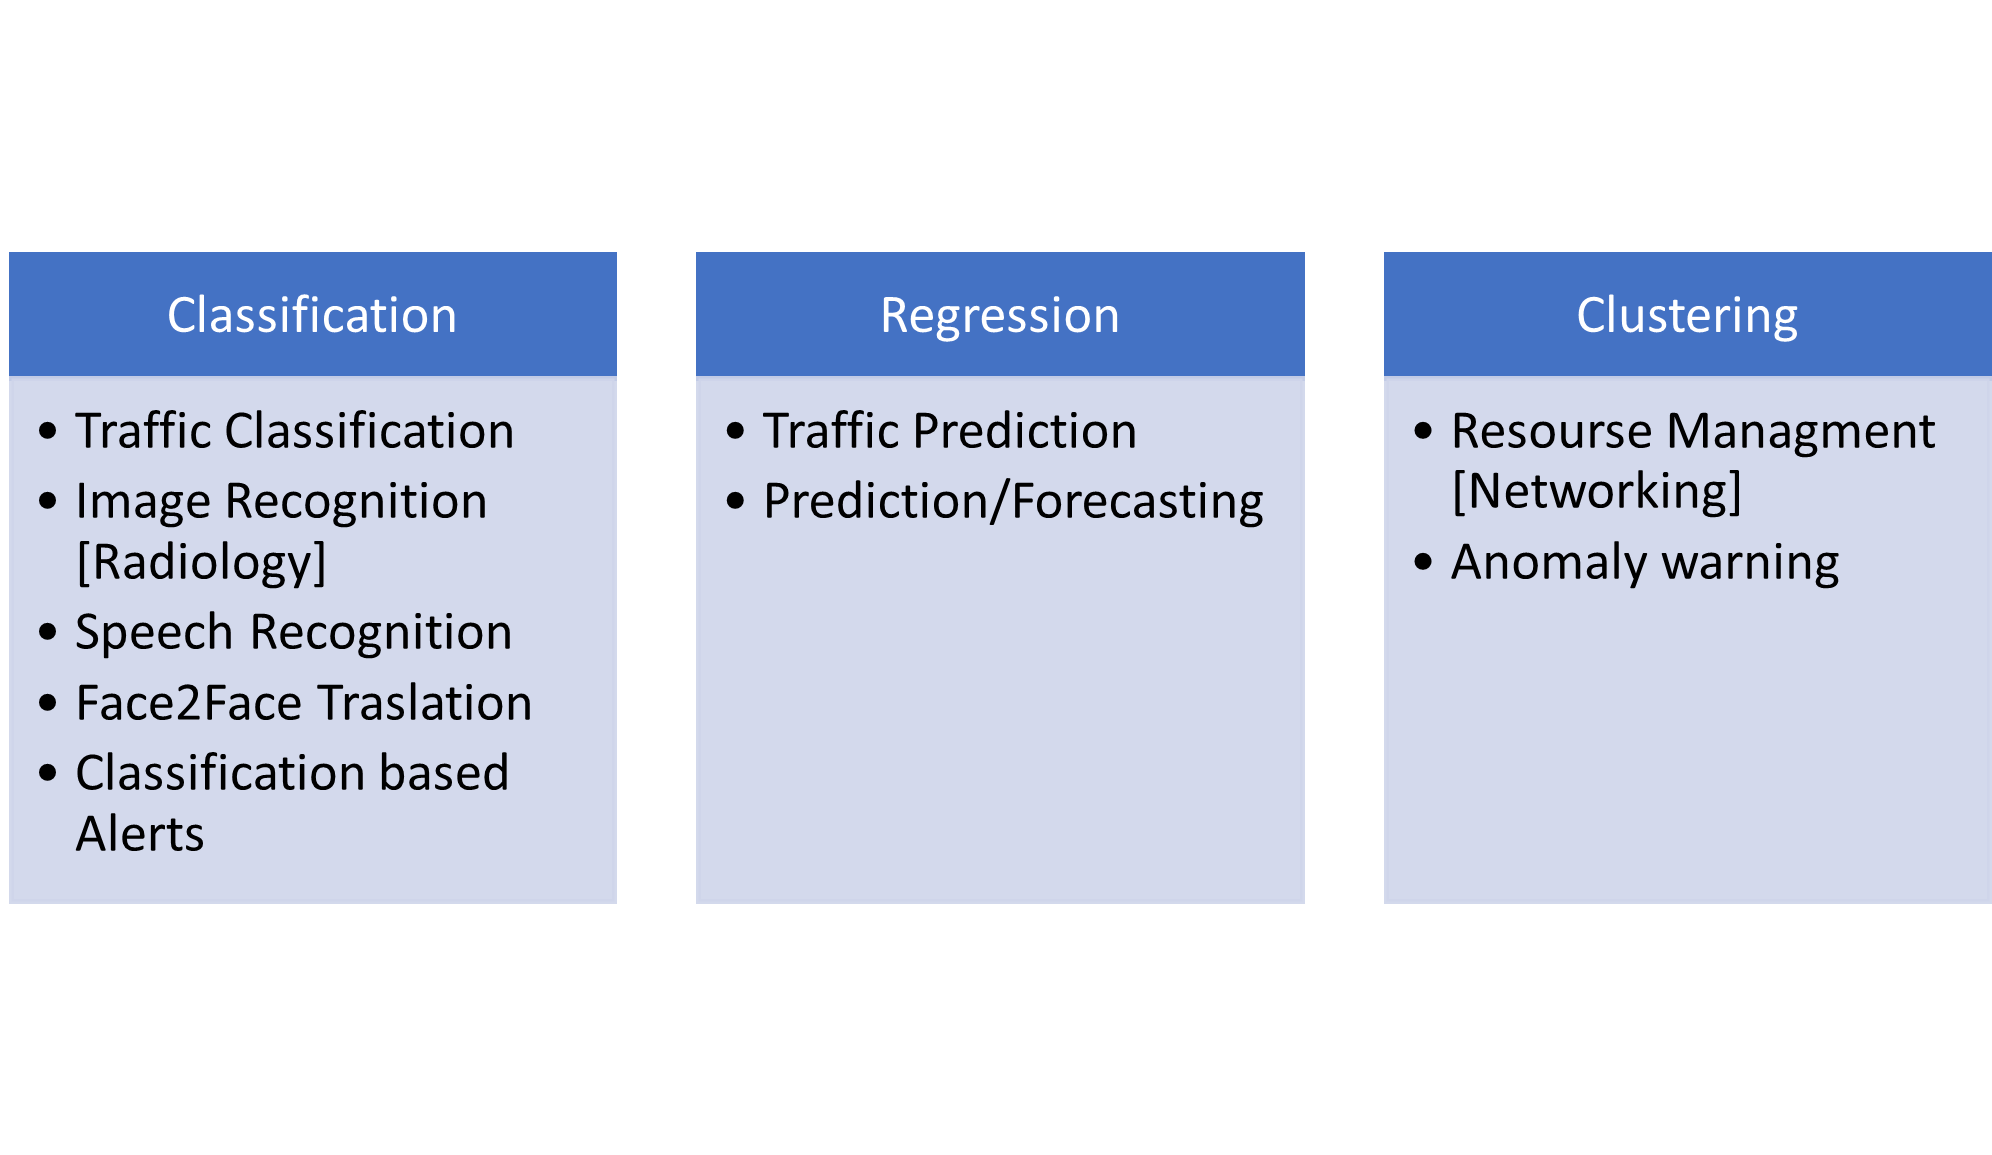
\includegraphics{categoryML.png}
  \caption{Partition ML Problem} 
  \end{figure}
\newpage
  \section{Conclusioni}
\begin{figure}[htbp]
  \centering
  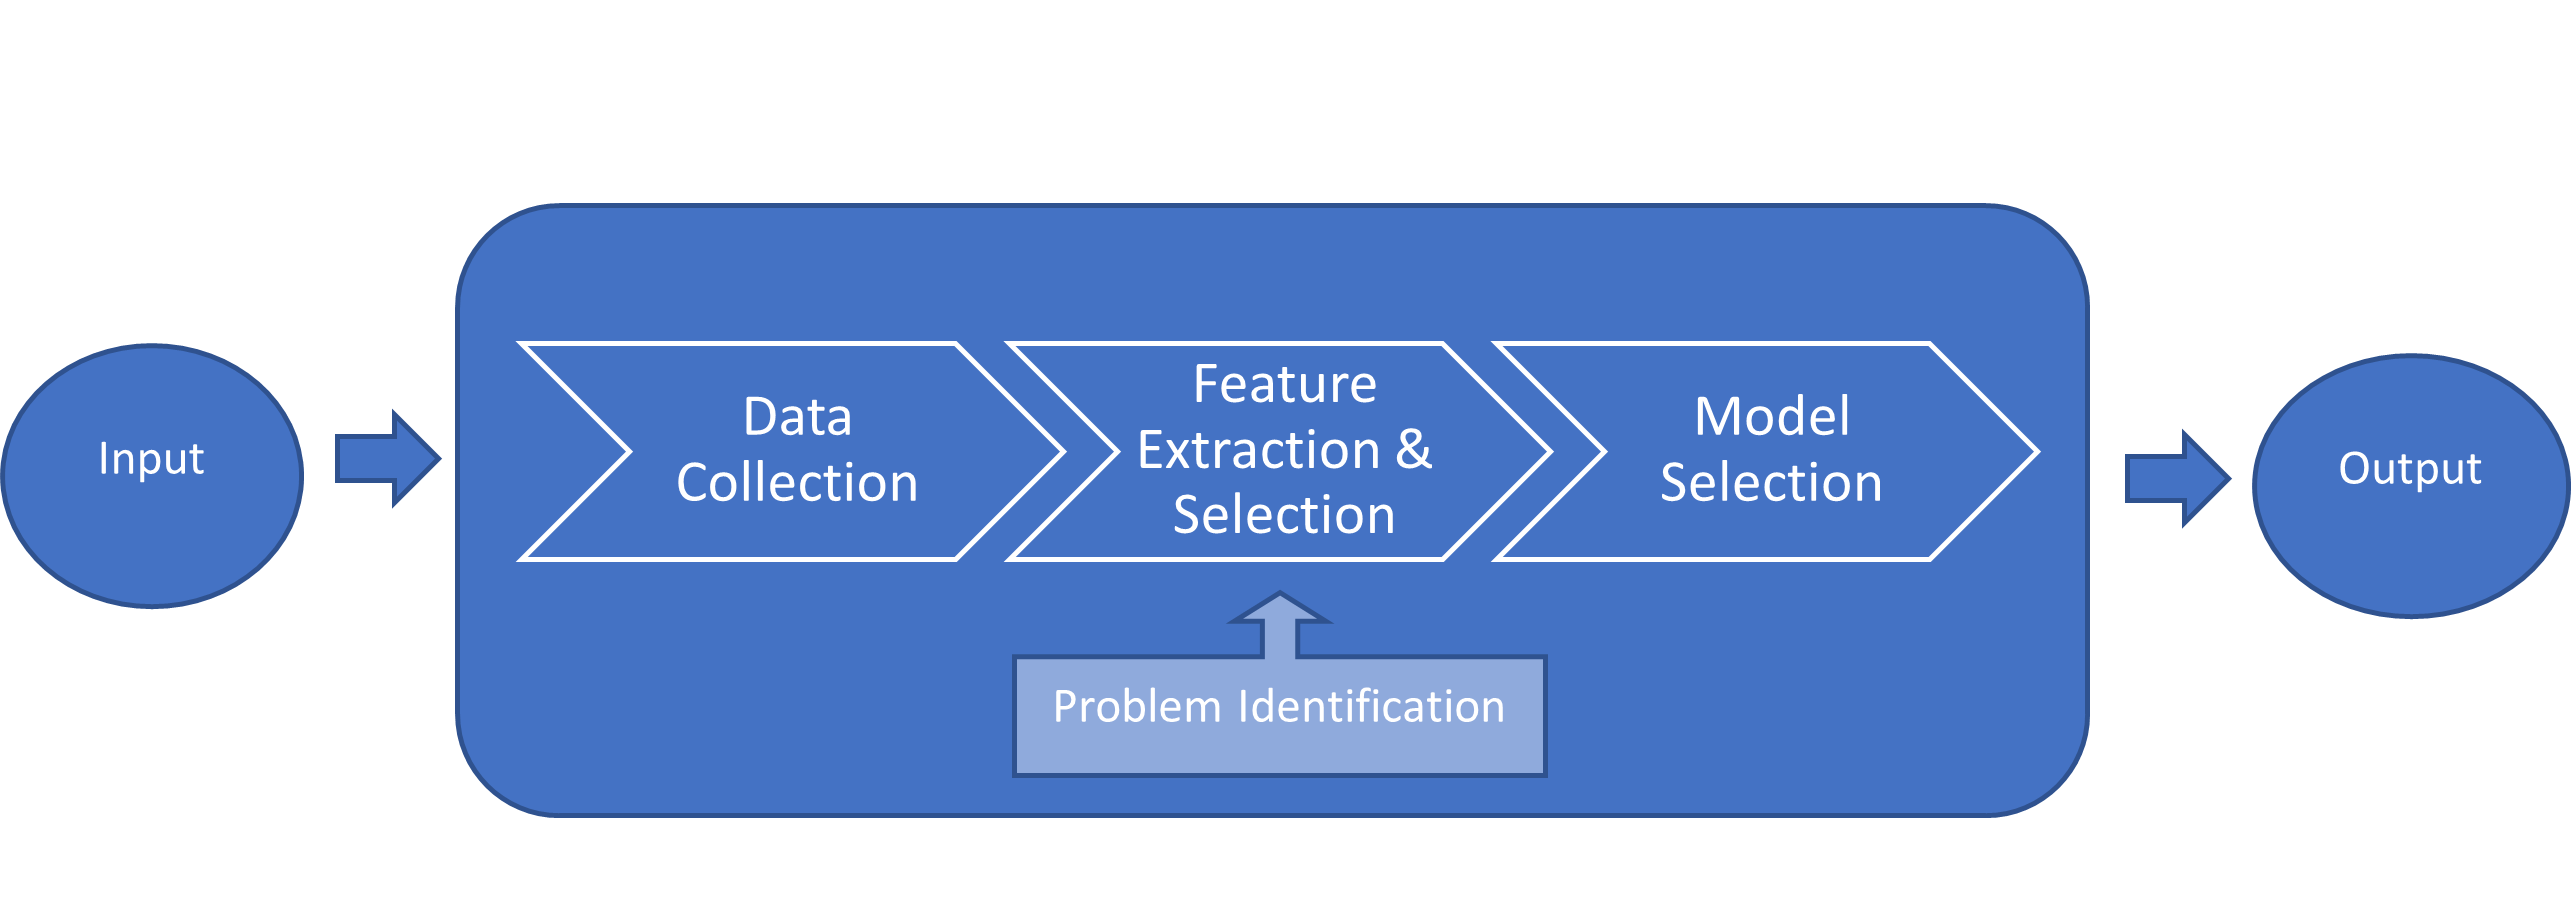
\includegraphics[width=.9\textwidth]{Immagine3.png} 
  \end{figure}
Concludendo cerchiamo di astrarre i nostri problemi evidenziando un pattern generico di invarianza tra i passaggi elencati nei capitoli precedenti.\\
Come notiamo nello schema, i 3 passaggi che diventano fondamentali cercando di automatizzare un processo di ML sono:
\begin{enumerate}
  \item Raccolta Dati
  \item Estrazione dai Dati 
  \item Selezione del Modello
\end{enumerate}
Come abbiamo detto in precedenza la raccolta dati è uno dei tasselli fondamentali, in seguito l’individuazione del problema rende possibile un'estrazione e una selezione dei dati piú completa, cercando di ottenere un insieme conforme al problema che ci troviamo a svolgere.\\
Una volta individuato il problema e raccolto i dati necessari in input, si proverá a selezionare in maniera automatica il modello adatto per prendere in input la mole di dati individuata.\\
Il modello preso in input i dati, restituirà il risultato che sarà l’output risultante da tutto il processo.\\
L’unica tolleranza la possiamo individuare nell’identificazione del problema, che in alcuni casi necessiterà di un intervento manuale; ad esempio, nel forecasting le tecniche predittive sono assai diverse, abbiamo bisogno di qualche indizio in più su quale modello selezionare.\\
L’efficienza di questo processo, soprattutto nell’identificazione del problema e la selezione del modello, già scarsa nei singoli flussi di lavoro del ML, si ritrova un peggioramento notevole dovuto all’identificazione del problema e alla scelta del modello di riferimento.
\end{document}